\lecture{5. I Was Their Husband}{05}

%------------------------------------------------------------------------------
\section{Introduction}

%--------------------------------------
\begin{frame}{A Husband in the Wild}
\begin{center}
	
\includegraphics[width=0.8\textwidth]{figures/lazyHusband.jpg}
\end{center}

\note{09:30}
\note[item]{Today we talk about God being our husband.}
\note[item]{Your husband may be this guy.}
\note[item]{That's not what God is.}
\note[item]{God's a perfect husband to His people}
\note[item]{And, as our loving husband He tries to persuade us to love Him back}
\end{frame}

%--------------------------------------
\begin{frame}{God wants a relationship with people}
\framesubtitle{Jeremiah 31:31-34}
	\keyversehiglight{I was their husband}
	
\note{09:33}
\note[item]{I will be their God, and they will be my people}
\note[item]{God has always made covenants (with responsibilities, and rewards) with us as a guarantee of our relationship with Him.}
\note[item]{One modern covenant we think about is marriage.  And, indeed, God sees himself as our husband, in both the OT and the NT (through Jesus).}6
\end{frame}

%--------------------------------------
\begin{goals}
\goal Examine what a husband is and how God is a husband to His people
\goal Elaborate on how God's love motivates us
\goal Consider practical ways to recognize and respond to God's love

\note{09:36}
\note[item]{Today we talk about, what God meant when he said He was husband to the children of Israel.}
\note[item]{We'll start by examining the marriage relationship in general.}
\note[item]{In some ways it seems like God created marriage just so he could show us how He loves us.}
\note[item]{And, while much of God's love was made available long before we could ever return love to him\ldots}
\note[item]{He still hopes that his love can motivate us to love Him back and to follow Him.}
\note[item]{We need to sensitive in listening to God's call and responding to it.}
\end{goals}

%------------------------------------------------------------------------------
\section{God has a husband's love}

%--------------------------------------
\begin{frame}{Marriage \emph{is} love}
\framesubtitle{Genesis 2:20-24}

\begin{columns}[c]
\begin{column}{0.6\textwidth}
	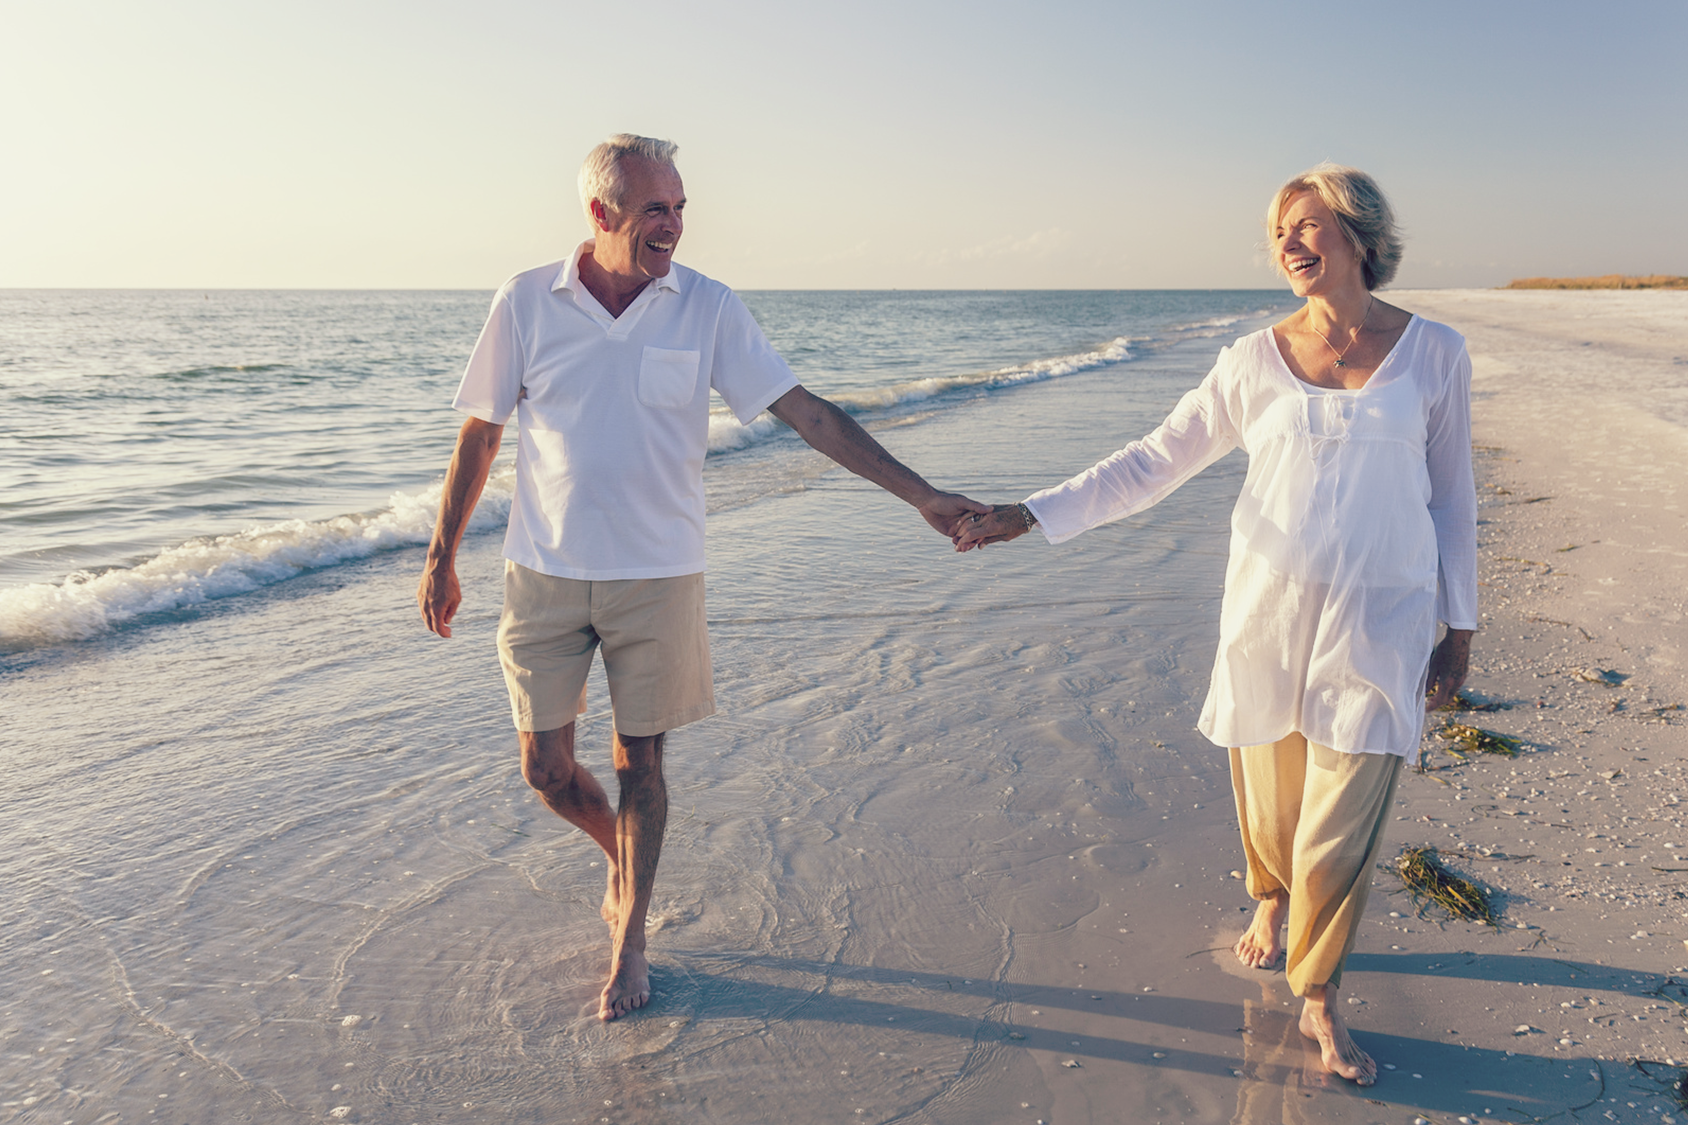
\includegraphics[width=\columnwidth]{figures/companionship.png}
\end{column}
\begin{column}{0.4\textwidth}
	The first marriage had\ldots
	\begin{itemize}
		\item Companionship
		\item Closeness
		\item Commitment
	\end{itemize}
\end{column}
\end{columns}

\note{09:38}
\note[item]{\textbf{Companionship:}}
\note[item]{Initially, man was alone (v20)}
\note[item]{He needed a helper (v20)}
\note[item]{\textbf{Closeness:}}
\note[item]{She was created from his rib -- 'bone of my bone' (v21-23)}
\note[item]{This is similar to God who created man in His image (Gen. 1:26)}
\note[item]{\textbf{Commitment:}}
\note[item]{Leave father and mother and cleave to his wife (v24)}
\end{frame}

%--------------------------------------
\begin{frame}{God was husband to the Israelites}
\framesubtitle{Jer. 31:32}

\begin{columns}[c]
\begin{column}{0.4\textwidth}
	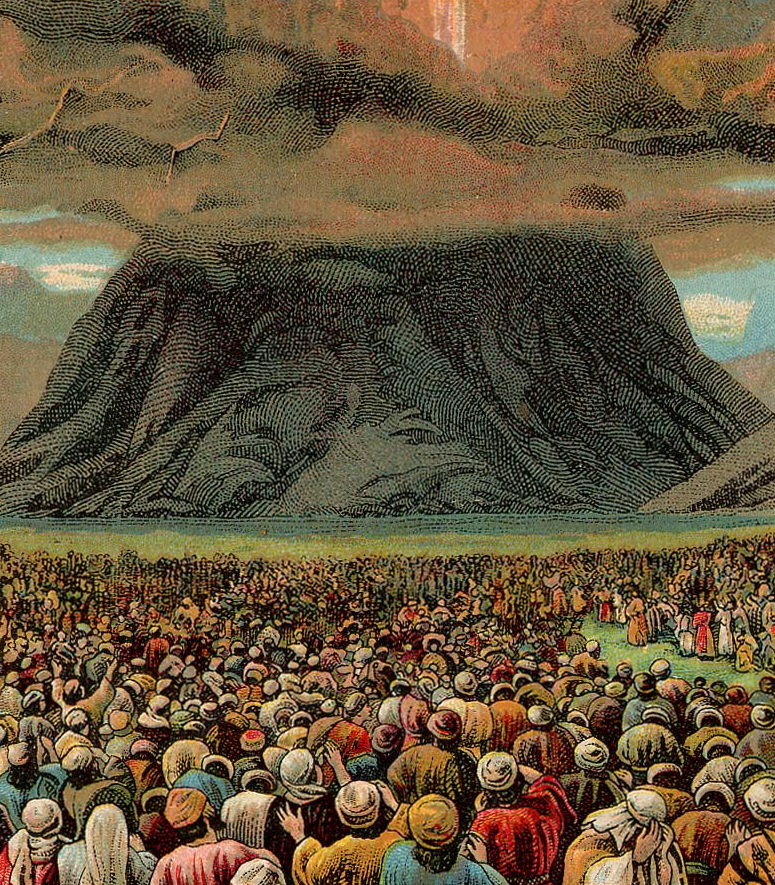
\includegraphics[width=\columnwidth]{figures/mountSinai.jpg}
\end{column}
\begin{column}{0.6\textwidth}
	\begin{itemize}
		\item Unlike human husbands,\\God's love is perfect\\{\footnotesize(Matt. 7:9-11, Heb. 12:11)}
    \item God offered Israel a direct relationship at Mt. Sinai\\{\footnotesize(Ex. 20:18-21)}
		\item The Israelites were afraid and refused.
	\end{itemize}
\end{column}
\end{columns}

\note{09:41}
\note[item]{If your son asks for bread, you wouldn't give him a stone (Matt 7:9-11)}
\note[item]{Earthly Fathers discipline as they see fit, God disciplines for our good. (Heb 12:11)}
\note[item]{Of course, the same would apply to God's role as husband to the Israelites.}
\note[item]{And, while we say that the trappings of the Old Law provided a separation between God and the Israelites\ldots}
\note[item]{God initially tried to communicate His will directly to them at Mt. Sinai.}
\note[item]{God came to them in all His holiness, on purpose, I'm sure, and the people of Israel were afraid.}
\note[item]{I suppose that's unsurprising.}
\note[item]{God continued to love Israel like a husband, even though they refused His initial offer.}
\end{frame}

%--------------------------------------
\begin{frame}{Christ is husband to the Church}
\framesubtitle{Heb 12:2, Eph 5:25}

\begin{columns}[c]
\begin{column}{0.5\textwidth}
	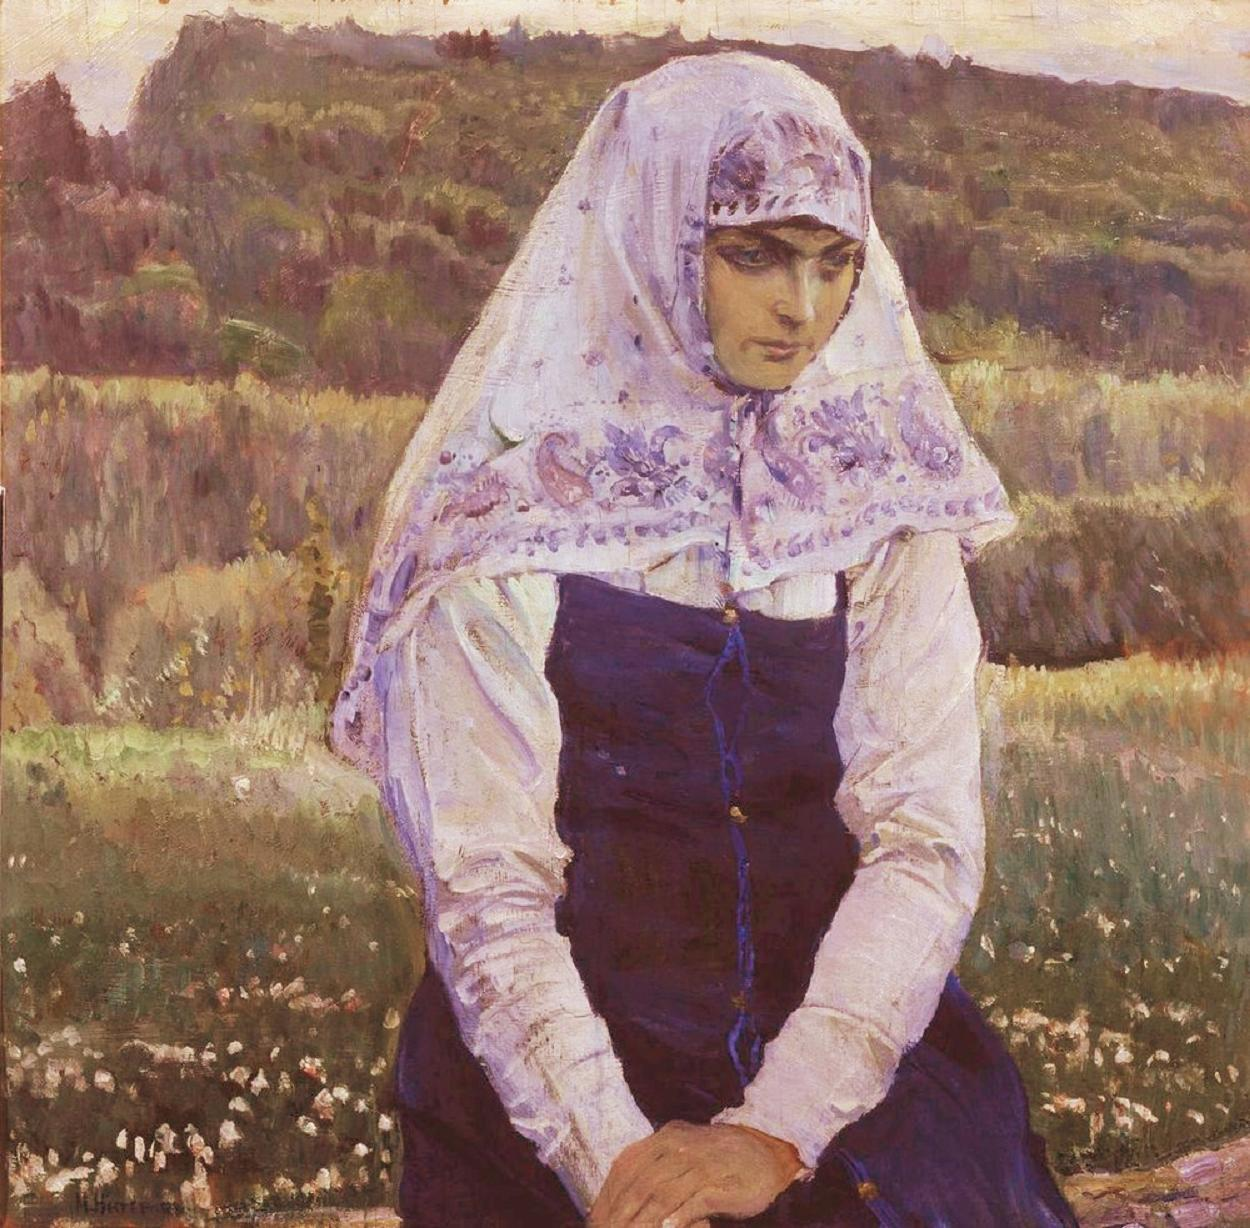
\includegraphics[width=\columnwidth]{figures/brideOfChrist.jpg}
\end{column}
\begin{column}{0.5\textwidth}
	Headship means sacrifice.  Jesus \ldots
	\begin{itemize}
    \item `Endured the cross'
    \item `Despised the shame'
    \item `Hostility against himself'
	\end{itemize}
\end{column}
\end{columns}

\note{09:45}
\note[item]{'Husbands, love your wives, as Christ loved the church and gave himself up for her,' Eph. 5:25}
\note[item]{Headship is really about sacrifice on the part of the husband}
\note[item]{Look at all the things Jesus did for the church}
\note[item]{He could have come to earth and \emph{demanded} respect from people}
\note[item]{But he wanted us to choose Him voluntarily (as we've already studied).}
\note[item]{Some men worry a lot about respect.}
\note[item]{And, they don't worry enough about companionship.}
\end{frame}


%------------------------------------------------------------------------------
\section{God tries to motivate us with love}

%--------------------------------------
\begin{frame}{You can't make someone love you,\\but you can try and persuade}
\begin{columns}[c]
\begin{column}{0.5\textwidth}
	
\includegraphics[width=\columnwidth]{figures/rose.jpg}
\end{column}
\begin{column}{0.5\textwidth}
	We all do this in marriage
	\begin{itemize}
    \item Things you give\ldots
		\begin{itemize}
			\item Communication
			\item Kindness
			\item Work around the house
      \item Take care of the kids
			\item Do your job(s)
			\item etc.
		\end{itemize}
    \item Responses you want\ldots
		\begin{itemize}
      \item Appreciation
      \item Kindness
      \item Closeness
			\item etc.
		\end{itemize}
	\end{itemize}
\end{column}
\end{columns}

\note{09:48}
\note[item]{Just as Jesus sacrificed Himself for us when we He wasn't loved in return, we should also give unselfishly to our spouse.}
\note[item]{Just like Jesus, though, we can hope that by our loving deeds, love will be returned.}
\note[item]{We do the same thing in marriage.}
\note[item]{God uses his acts of love to try and motivate us to love Him back, to live righteously, and to endure in our faith.}
\end{frame}

%--------------------------------------
\begin{frame}{Jesus' sacrifice motivates us}
\framesubtitle{Heb. 12:1-4}
\begin{columns}[c]
\begin{column}{0.4\textwidth}
	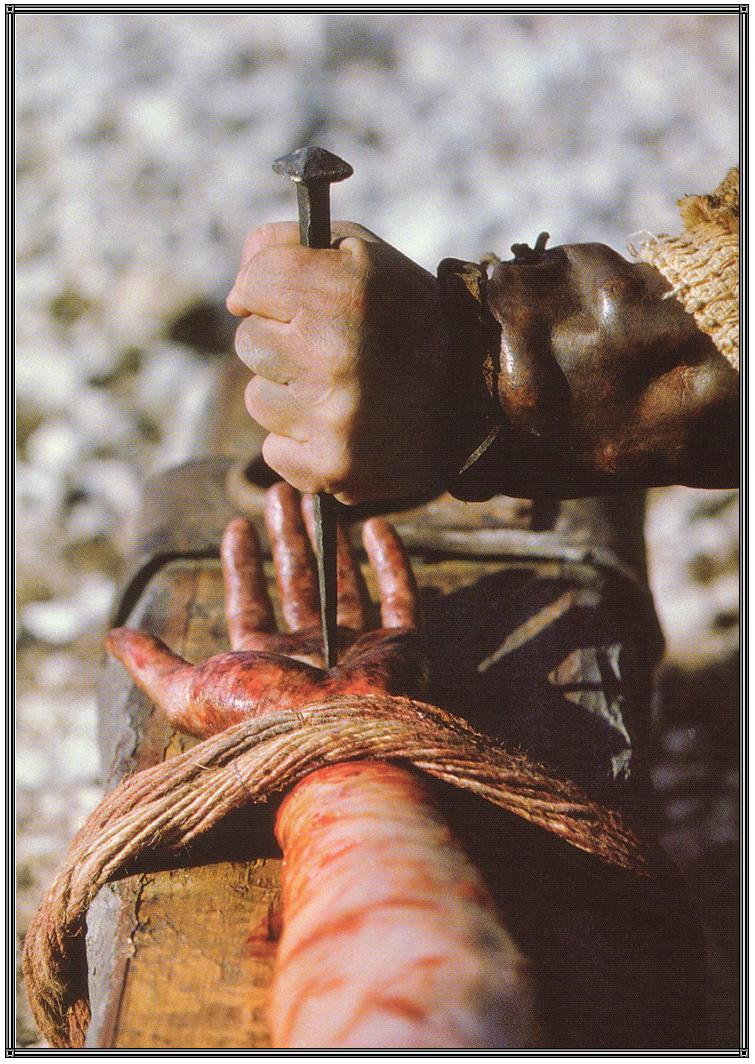
\includegraphics[width=\columnwidth]{figures/nailedToTheCross.jpg}
\end{column}
\begin{column}{0.6\textwidth}
	\begin{itemize}
		\item Gifts
		\begin{itemize}
			\item Endured the cross
			\item Ignored the shame
			\item Endured hostilities from sinners
		\end{itemize}
		\item Response
		\begin{itemize}
			\item Do not grow weary or faint-hearted
		\end{itemize}
	\end{itemize}
\end{column}
\end{columns}

\note{09:51}
\note[item]{We turn to the big passage in our reading.}
\note[item]{Previously, in chapter 11, the writer recounted a host of people who lived faithfully and says, 'run with endurance'}
\note[item]{Now, the writer turns us toward Jesus, whose love for us should motivate us to be strong and courageous in the face of persecution.} 
\end{frame}

%--------------------------------------
%\begin{frame}{God, as our Father, motivates us with discipline}
%\framesubtitle{Heb. 12:5-11}
%\begin{columns}[c]
%\begin{column}{0.3\textwidth}
	%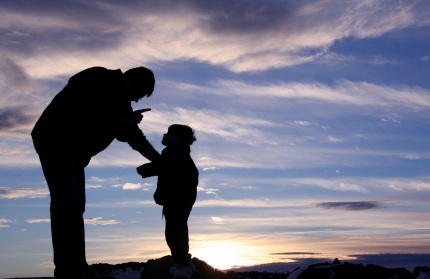
\includegraphics[width=\columnwidth, trim=0 0 200px 0, clip=true]{figures/discipline.jpg}
%\end{column}
%\begin{column}{0.7\textwidth}
	%\begin{itemize}
		%\item God's discipline works in many areas.
		%\begin{itemize}
			%\item Discipline \emph{is} love 
			%\item It's not just consequences.
			%\item In Hebrews it's persecution.
		%\end{itemize}
		%\item Our response
		%\begin{itemize}
      %\item The peaceable fruit of righteousness
      %\item Be strong and courageous
      %\item Make straight paths for your feet
      %\item Strive for peace with everyone
      %\item Strive for holiness
      %\item Avoid the 'root of bitterness'
      %\item Avoid sexual immorality 
		%\end{itemize}
	%\end{itemize}
%\end{column}
%\end{columns}
%
%\note{09:54}
%\note[item]{We think about discipline with regard to making mistakes}
%\note[item]{They were being disciplined with persecution, which was not their fault}
%\end{frame}

%--------------------------------------
\begin{frame}{God, the husband, tried to motivate the children of Israel}
\framesubtitle{Heb. 12:18-21}
\begin{columns}[c]
\begin{column}{0.5\textwidth}
	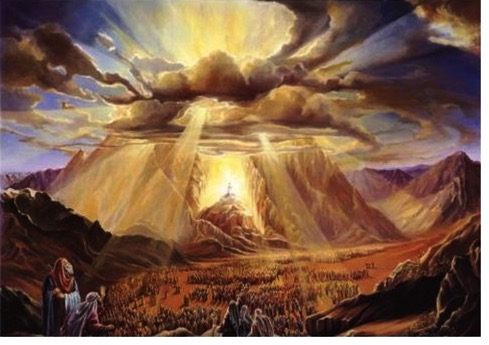
\includegraphics[width=\columnwidth]{figures/mountSinai2.jpg}
\end{column}
\begin{column}{0.5\textwidth}
	\begin{itemize}
		\item Gifts
		\begin{itemize}
			\item Mt. Sinai direct relationship
      \item Emphasized that God is holy
      \item The Old Law
      \item Physical Blessing
		\end{itemize}
		\item Response
    \begin{itemize}
		  \item Love
			\item Obedience
			\item Faithfulness
    \end{itemize}
	\end{itemize}
\end{column}
\end{columns}
\begin{center}
But, they were too afraid of God to listen to Him!
\end{center}
\note{09:55}
\note[item]{There's a good illustrations of freezing up here.}
\note[item]{I never thought that people actually give up.}
\note[item]{But, they do all the time}
\note[item]{Reminds me of the parable of the talents and the man who hid is talent in the ground.}
\note[item]{There's certainly a part of this that's on purpose.  We need a dichotomy between the Old and New Covenants.}
\end{frame}

%--------------------------------------
\begin{frame}{God, the  husband, motivates Christians}
\framesubtitle{Heb. 12:18-24}
\begin{columns}[T]
\begin{column}{0.5\textwidth}
	Gifts -- Spiritual Mt. Zion
    \begin{itemize}
      \item Pleasant and happy
      \item Innumerable angles in festal gathering
      \item Assembly of the firstborn
      \item Spirits of the righteous made perfect by Jesus
      \item Jesus, and His blood which is MORE innocent than the blood of Able
      \item Grace (v 15)
		\end{itemize}
	%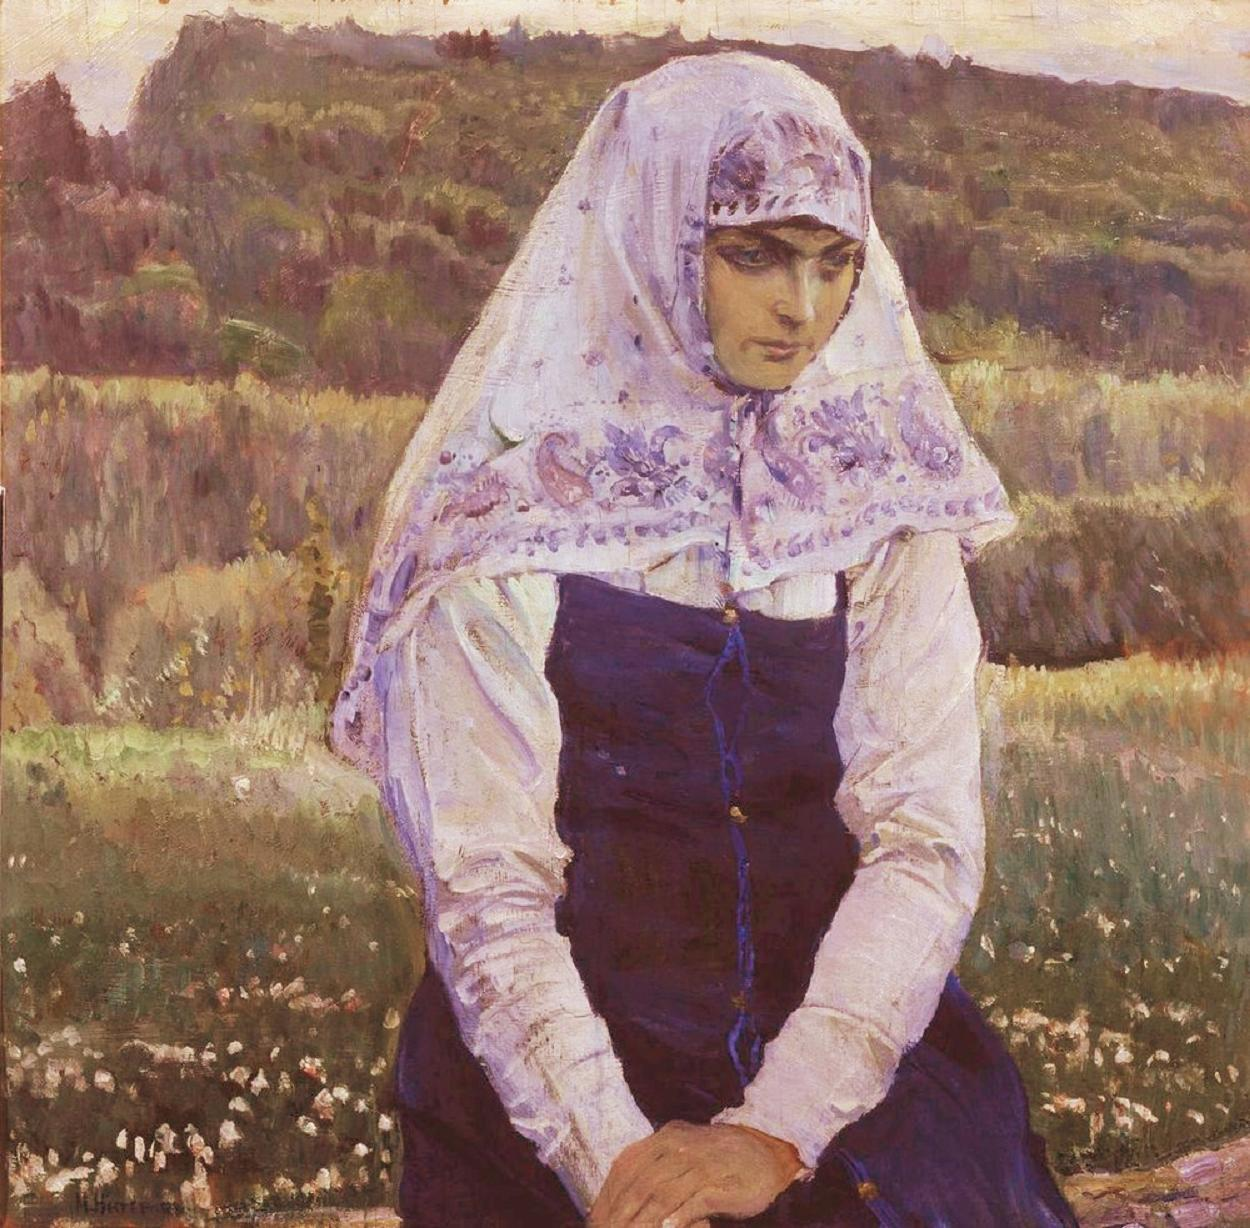
\includegraphics[width=\columnwidth]{figures/brideOfChrist.jpg}
\end{column}
\begin{column}{0.5\textwidth}
	Response
	\begin{itemize}
			\item Don't refuse Him
      \item Thankfulness for a unshakeable kingdom
      \item Reverence and awe
		\end{itemize}
\end{column}
\end{columns}

\note{09:58}
\note[item]{God's revelation of Himself at Mt. Sinai was terrifying.}
\note[item]{It was the same for Isaiah, and really the same for John.}
\note[item]{If you had to stand before God by yourself, you'd be afraid, too.}
\note[item]{But, unlike the children of Israel, we have Jesus.}
\note[item]{So, coming to Mount Zion is a happy and wonderful thing.}
\end{frame}

%------------------------------------------------------------------------------
\section{Recognize and respond to God's love}

%--------------------------------------
\begin{frame}{God's love shown in Jesus}
\framesubtitle{I John 4:9-10}
\begin{columns}[c]
\begin{column}{0.5\textwidth}
	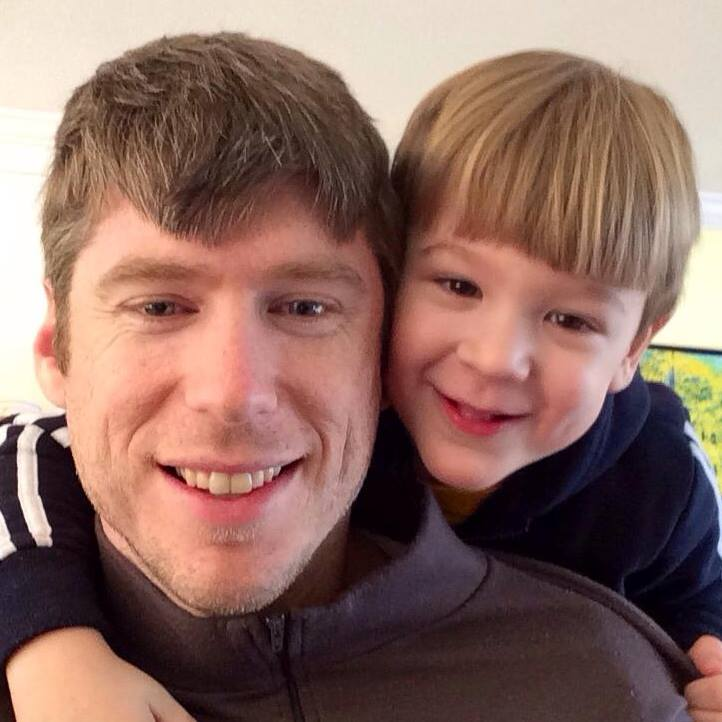
\includegraphics[width=\columnwidth]{figures/toddAndEzra.jpg}
\end{column}
\begin{column}{0.5\textwidth}
	\begin{itemize}
    \item Gave His own Son \ldots
    \item When we didn't love him back.
	\end{itemize}
\end{column}
\end{columns}

\note{10:03}
\note[item]{Needed an excuse to show this picture, again}
\note[item]{Just replace this, in your mind, with you and your own Son}
\note[item]{That's a sacrifice.}
\end{frame}

%--------------------------------------
\begin{frame}{Our response to God's love}
\framesubtitle{I John 4:7-12}
\begin{columns}[c]
\begin{column}{0.5\textwidth}
	
\includegraphics[width=\columnwidth]{figures/doSomething.jpg}
\end{column}
\begin{column}{0.5\textwidth}
	\begin{itemize}
    \item Love God back
    \item Love the brethren
    \item Then we know God
	\end{itemize}
\end{column}
\end{columns}

\note{10:04}
\note[item]{Left out `keep His commandments'. But, that's in other parts of I John.}
\end{frame}

%--------------------------------------
\begin{frame}{Questions for us}
	\centering
	\begin{itemize}
    \item Am I listening for the ways God is loving me?
    \item Am I sensitive in responding to God's Love?
	\end{itemize}
\note{10:06}
\note[item]{Can you think of some other places we see God's love?}
\note[item]{How does it motivate you?}
\end{frame}
%------------------------------------------------------------------------------
\section{Review}

\begin{frame}{I was a husband to them}
	\begin{itemize}
		\item God loves his people as a husband loves his wife
		\item His love should motivate us to live righteous
		\item We need to see God's love in our everyday life
		\item We need to keep our heart softened so we can feel and respond to God's love.
	\end{itemize}
	
\note{10:12}
\note[item]{Israel was unfaithful.}
\note[item]{We'll discuss that next week in `My covenant they broke'}
\end{frame}